\documentclass[final]{beamer}

% ====================
% Packages
% ====================

\usepackage[T1]{fontenc}
\usepackage[utf8]{luainputenc}
\usepackage{lmodern}
\usepackage[size=custom, width=122, height=91, scale=1.2]{beamerposter}
\usetheme{gemini}
\usecolortheme{msu}
\usepackage{graphicx}
\usepackage{booktabs}
\usepackage{tikz}
\usepackage{pgfplots}
\pgfplotsset{compat=1.14}
\usepackage{anyfontsize}

% ====================
% Custom Title Styling
% ====================

\definecolor{myblue}{RGB}{10,30,70}    % dark blue background
\definecolor{myyellow}{RGB}{255,215,0} % golden yellow title text

% Regular block styling
\setbeamercolor{block title}{fg=myyellow,bg=myblue}
\setbeamerfont{block title}{series=\bfseries,size=\Large}
\setbeamercolor{block body}{bg=white,fg=black}

% Alert block styling
\setbeamercolor{block title alerted}{fg=myyellow,bg=myblue}
\setbeamerfont{block title alerted}{series=\bfseries,size=\large}
\setbeamercolor{block body alerted}{bg=white,fg=black}

% Example block styling
\setbeamercolor{block title example}{fg=myyellow,bg=myblue}
\setbeamerfont{block title example}{series=\bfseries,size=\huge}
\setbeamercolor{block body example}{bg=white,fg=black}

% Custom block title height and alignment (updated thickness)
\setbeamertemplate{block begin}{
  \vskip0.3em
  \begin{beamercolorbox}[rounded=true,center,shadow=false,dp=1.2ex,ht=3.2ex]{block title}
    \usebeamerfont*{block title}\insertblocktitle
  \end{beamercolorbox}
  {\parskip0pt\par}
  \usebeamercolor[fg]{block body}
  \usebeamerfont{block body}
  }


\setbeamertemplate{block end}{
\begin{beamercolorbox}[colsep*=.75ex,vmode]{block body}
  \end{beamercolorbox}
  \vspace{1em}
}


% ====================
% Lengths
% ====================

\newlength{\sepwidth}
\newlength{\colwidth}
\setlength{\sepwidth}{0.025\paperwidth}
\setlength{\colwidth}{0.3\paperwidth}

\newcommand{\separatorcolumn}{\begin{column}{\sepwidth}\end{column}}

\title{DeCLIP: Hard Negative Mining through Image Decomposition and Inpainting}

\author{Zhanhao Liu, Qiulin Fan, Huanchen Jia, Lingyu Meng}

\institute[shortinst]{Department of Mathematics $\&$ Department of Computer Science, University of Michigan}

% ====================
% Footer (optional)
% ====================

\footercontent{
  \href{https://github.com}{Github: https://github.com/SaddySamoyed/545-project} \hfill
Poster Session of CSE 545}
% (can be left out to remove footer)


% ====================
% Logo (optional)
% ====================

% use this to include logos on the left and/or right side of the header:
% Left: institution
 \logoright{
\includegraphics[height=5cm]{logos/blockM.png}}
% Right: funding agencies and other affilations 
%\logoright{\includegraphics[height=7cm]{logos/NSF.eps}}
% ====================
% Body
% ====================

\begin{document}

\begin{frame}[t]
\begin{columns}[t]
\separatorcolumn
\definecolor{myblue}{RGB}{10,30,70}    % dark blue background
\definecolor{myyellow}{RGB}{255,215,0} % golden yellow title text

\begin{column}{\colwidth}

    \begin{block}{Motivation}
    % Customize block title
    \setbeamercolor{block title}{fg=myyellow,bg=myblue}
    \setbeamerfont{block title}{series=\bfseries,size=\Large}
    \setbeamercolor{block body}{bg=white,fg=black}
    % Customize alertblock title
    \setbeamercolor{block title alerted}{fg=myyellow,bg=myblue}
    \setbeamerfont{block title alerted}{series=\bfseries,size=\large}
    \setbeamercolor{block body alerted}{bg=white,fg=black}

    % Customize exampleblock title
    \setbeamercolor{block title example}{fg=myyellow,bg=myblue}
    \setbeamerfont{block title example}{series=\bfseries,size=\large}
    \setbeamercolor{block body example}{bg=white,fg=black}

    Despite CLIP’s success in vision-language learning, it struggles with fine-grained understanding due to its reliance on global image-text alignment, limiting performance in tasks requiring subtle visual distinctions.

    \vspace{0.6em}
    \textbf{How can we push CLIP to better learn localized visual details?}

    Our project explores \textit{image-based hard negatives} as a way to enhance CLIP’s attention to fine-grained features and improve its robustness in real-world multimodal tasks. 

\begin{figure}
    \centering
    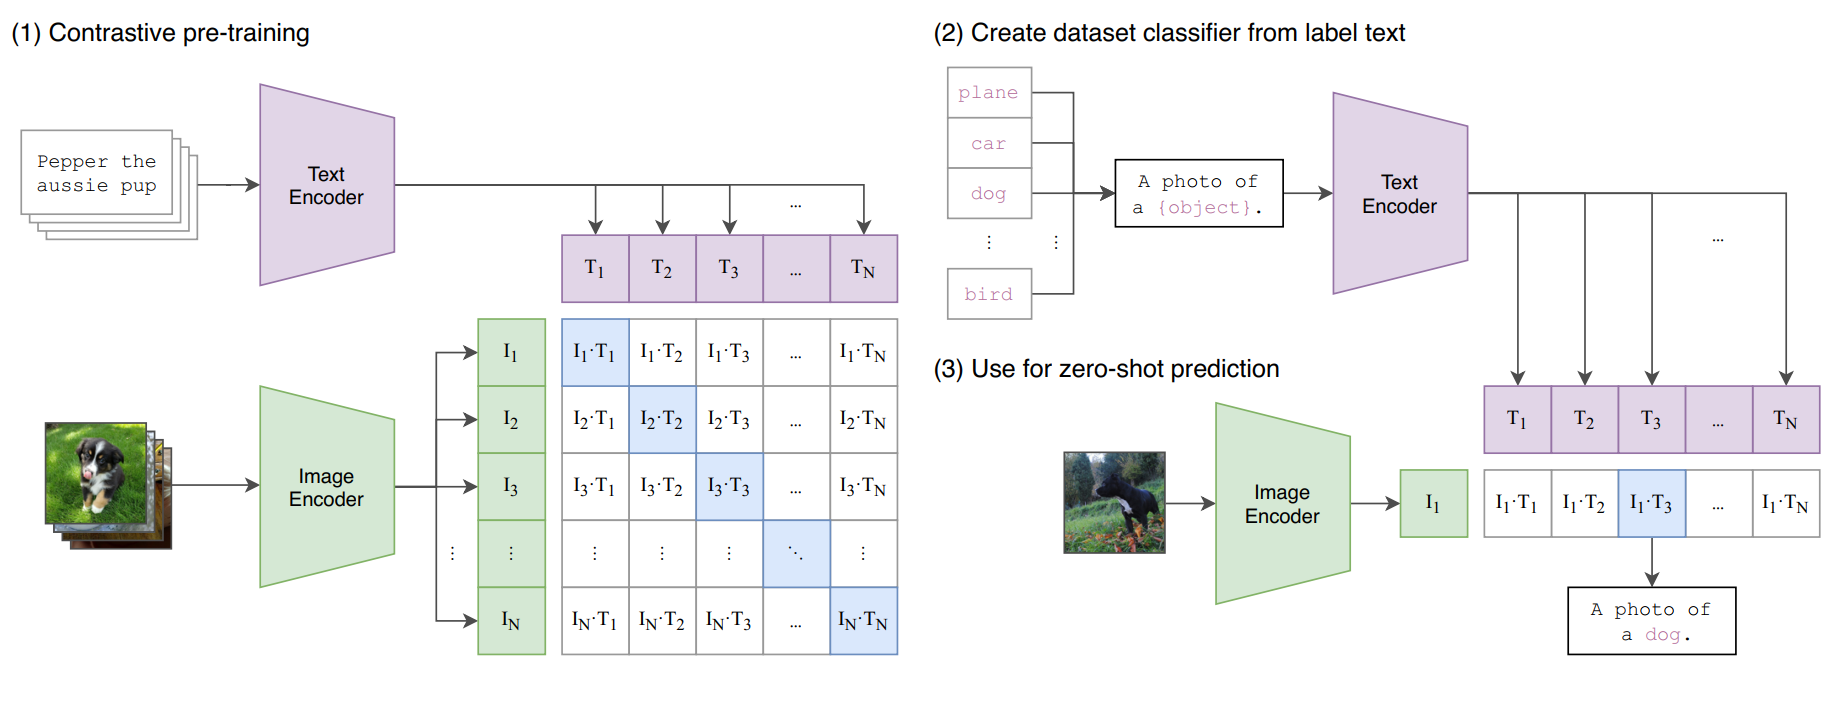
\includegraphics[width=1\linewidth]{poster/assets/openai_clip.png}
    \caption{Original CLIP Model}
    \label{fig:Original CLIP Model}
\end{figure}
\end{block}


 \begin{block}{Dataset and Preprocessing}
  \begin{itemize}
    \item \textbf{Dataset:} The MS COCO 2014 dataset containing 164{,}000 images (82{,}783 of which for training), and each image is paired with 5 captions. We use the first one for keyword extration and further rewriting.
    
    \item \textbf{Preprocessing for caption (Stage 1):} To guide DeClip’s visual–textual grounding, on the caption end, we preprocess each caption in two stages:\\
        \textbf{Keyphrase Extraction:} We parse each caption using a part‑of‑speech tagger and select the most salient nouns that denote primary objects or spatial relations, ensuring the model focuses on core scene elements.
        
        \textbf{Category Mapping:} Each extracted noun is translated into its corresponding YOLO detection category from the 80 classes defined in YOLOv8, allowing DeClip to leverage pretrained object‑detection priors and attend more to the difference of corresponding regions during training.
         \item \textbf{Preprocessing for image and caption (Stage 2):} We then use YOLOv8 to segment the image, generating masks. For keywords that generate empty masks, it means the keyword-category map is not correct, so we remove the keyword from the map.
  \end{itemize}
  \vspace{1em}
    \begin{figure}[htbp]
  \centering
  \begin{minipage}[t]{0.47\textwidth}
    \centering
    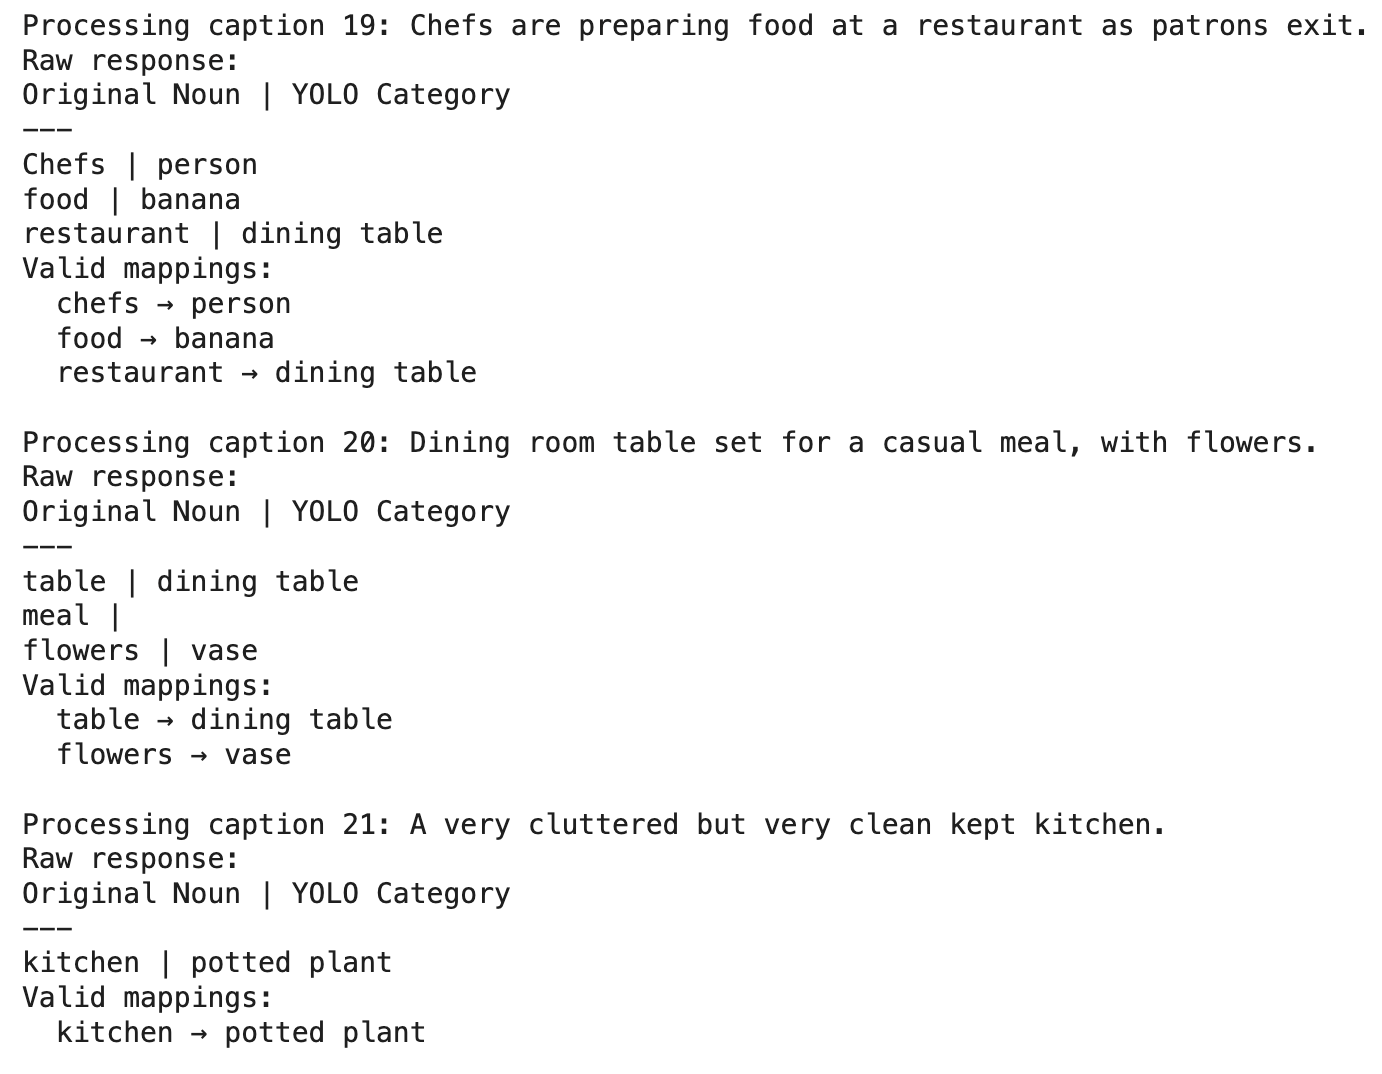
\includegraphics[width=\linewidth]{poster/assets/Screenshot 2025-04-22 at 20.16.18.png} % 替换为你的图片路径
    \caption{LLM keyword extration and mapping}
    \label{fig:img1}
  \end{minipage}
  \hfill
  \begin{minipage}[t]{0.5\textwidth}
                \centering
    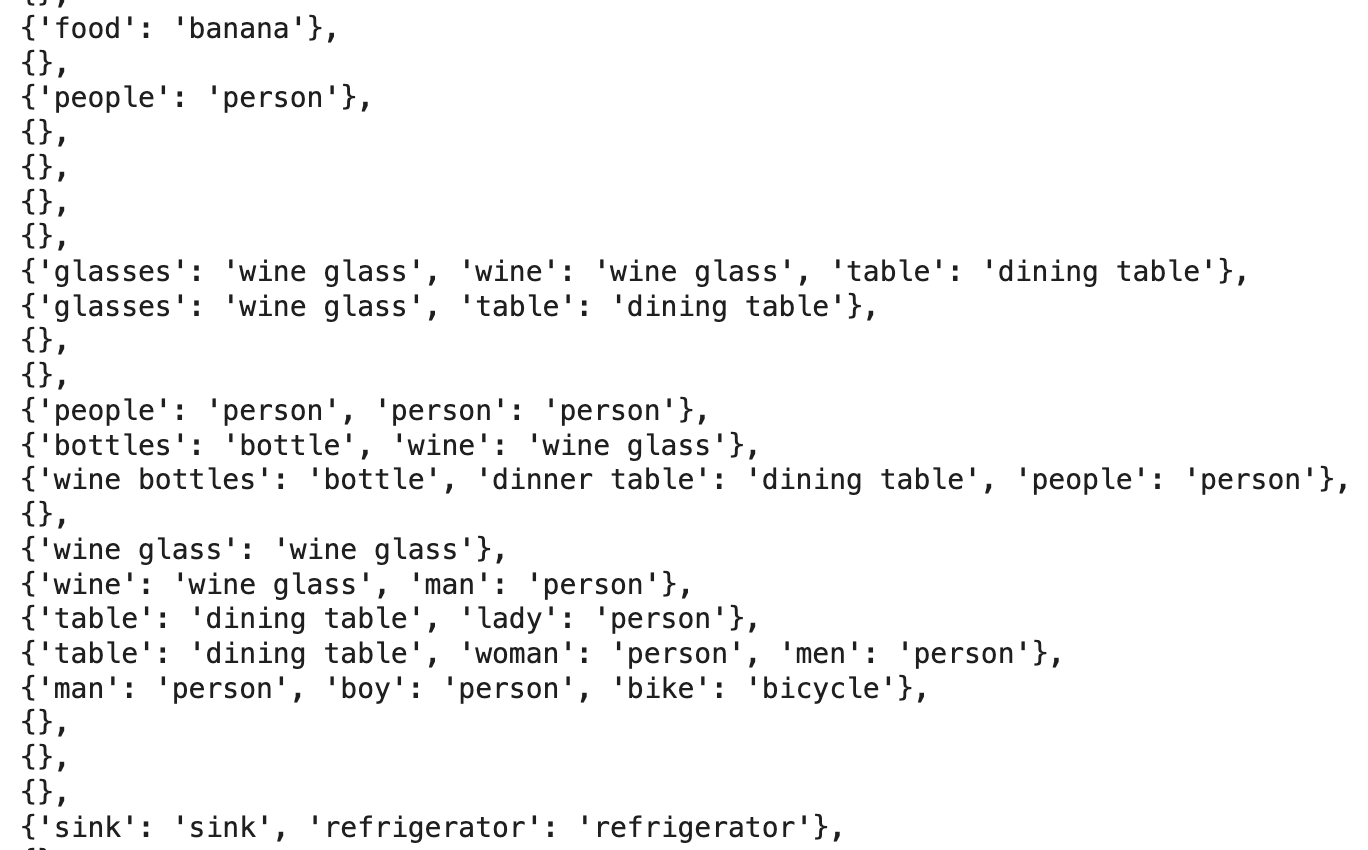
\includegraphics[width=\linewidth]{poster/assets/Screenshot 2025-04-23 at 07.34.33.png} % 替换为你的图片路径
    \caption{Updated keyword-category map after segmentation}
    \label{fig:img2}
  \end{minipage}
\end{figure}

\end{block}
\end{column}
\separatorcolumn

\begin{column}{\colwidth}

\begin{block}{Methodology}

We propose \textbf{DeCLIP}, a framework that improves fine-grained visual understanding by generating \textbf{hard negatives} on the \textit{image side}.

Given an image-text pair:
\begin{itemize}
    \item Remove key objects from the image to create a \textbf{dual image}, keeping the caption unchanged → a semantically mismatched hard negative.
    \item Remove corresponding keywords from the caption to create a \textbf{dual text} aligned with the altered image → a new positive pair.
\end{itemize}
Surely, dual images and original captions form false examples and almost surely, dual images and dual captions form negative examples. 
\vspace{0.5em}
\begin{alertblock}{Dual Image and Dual Text Generation}
\begin{enumerate}
    \item \textbf{Diffusion Inpainting:} Remove masked objects to generate \textbf{dual images.}
    \item \textbf{Caption Rewriting:} Use LLM to remove matched keywords, producing \textbf{dual texts}.
\end{enumerate}
\end{alertblock}

\textbf{Theoretical Motivation.} Based on the \textit{manifold hypothesis}, we assume:
\begin{itemize}
    \item Dual images/texts lie near originals in embedding space.
    \item This helps CLIP learn subtle mismatches and improves multimodal robustness.
\end{itemize}
\begin{figure}
    \centering
    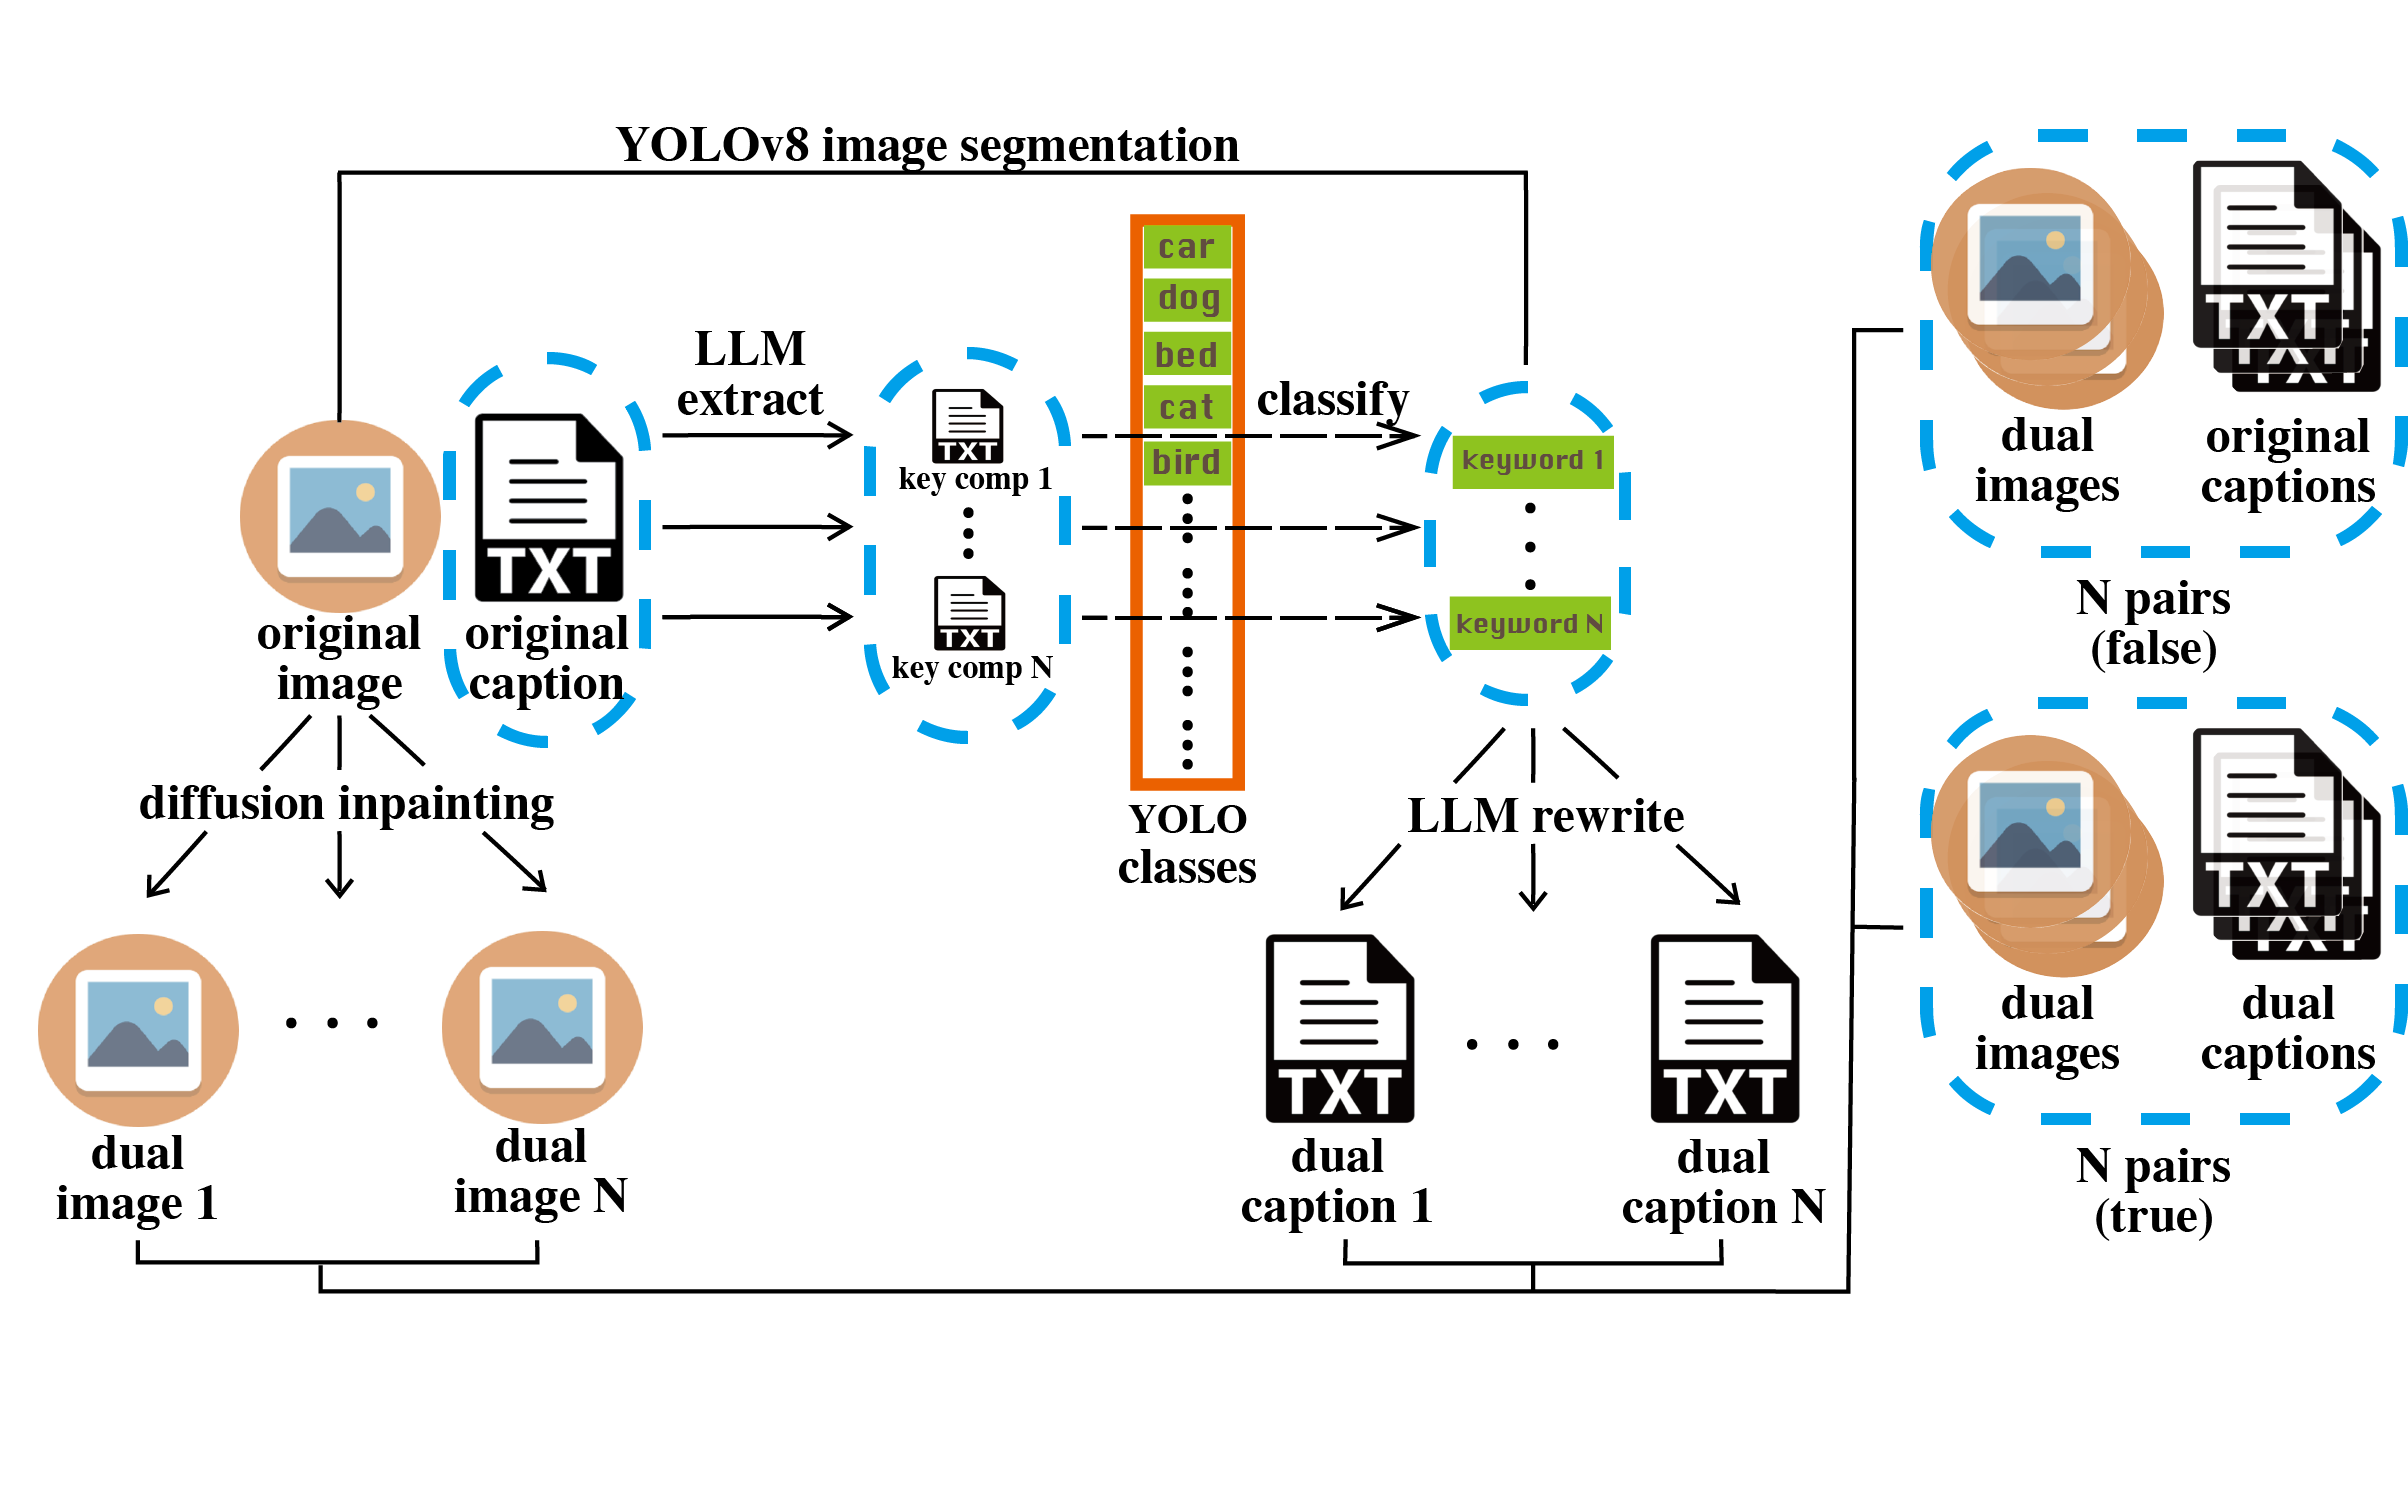
\includegraphics[width=0.9\linewidth]{poster/overall_method.png}
    \caption{Conceptual diagram of DeCLIP pipeline}
\end{figure}
\end{block}
\begin{block}{Training and Fine-tuning}
In this section, we evaluate our model using a \textbf{margin-based loss function}, which is an enhancement of the original CLIP loss. The loss for each example is defined as:
\[
\ell = \frac{1}{N} \sum_{j=1}^{N} \max\left(0,\; \text{MARGIN} + s_j^{-} - s^{+} \right)
\]
This formulation incorporates a margin term to enforce a minimum difference between positive and negative example scores. The use of the ReLU activation function ensures that only violations of this margin contribute to the loss. By averaging over all negative samples, the loss function emphasizes positive examples, encouraging the model to learn more discriminative features.
\end{block}

\end{column}

\separatorcolumn

  \begin{column}{0.3\textwidth}

\begin{block}{Result}

\begin{figure}
    \centering
    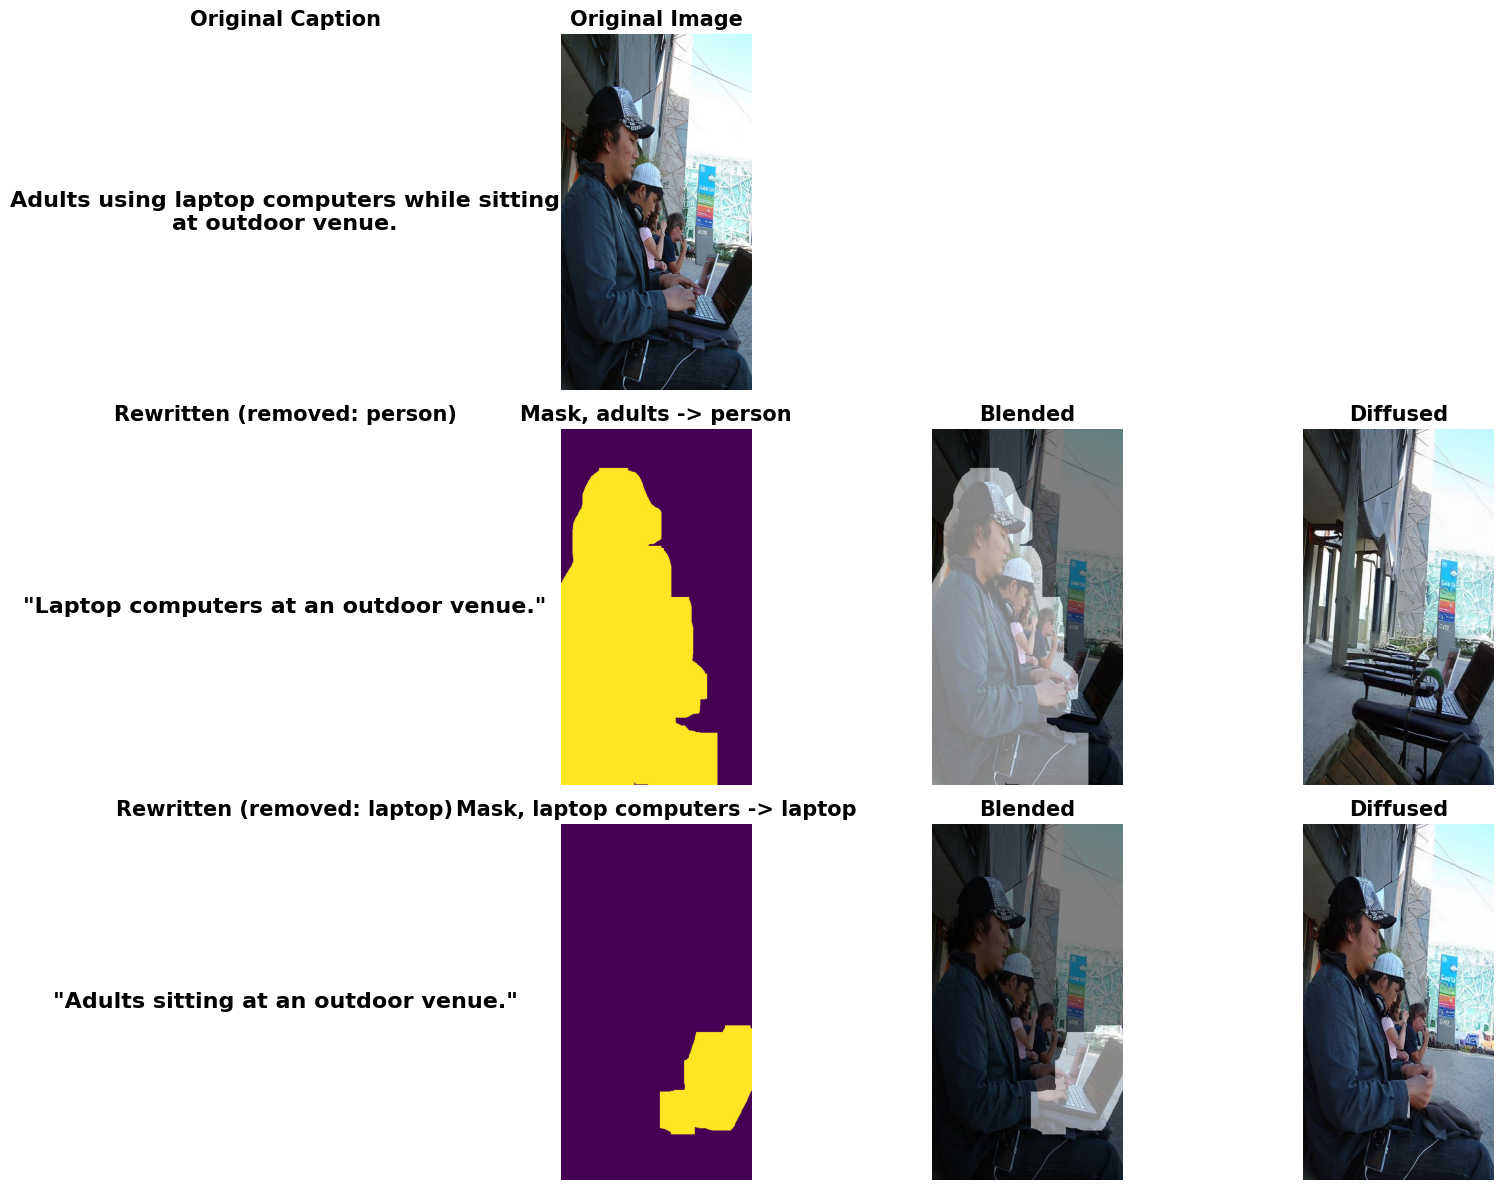
\includegraphics[width=0.8\linewidth]{poster/assets/preliminary.png}
    \caption{A random sample of dual (image, caption) pairs generated by Declip.}
\end{figure}
\begin{minipage}[t]{0.34\linewidth}
        \centering
        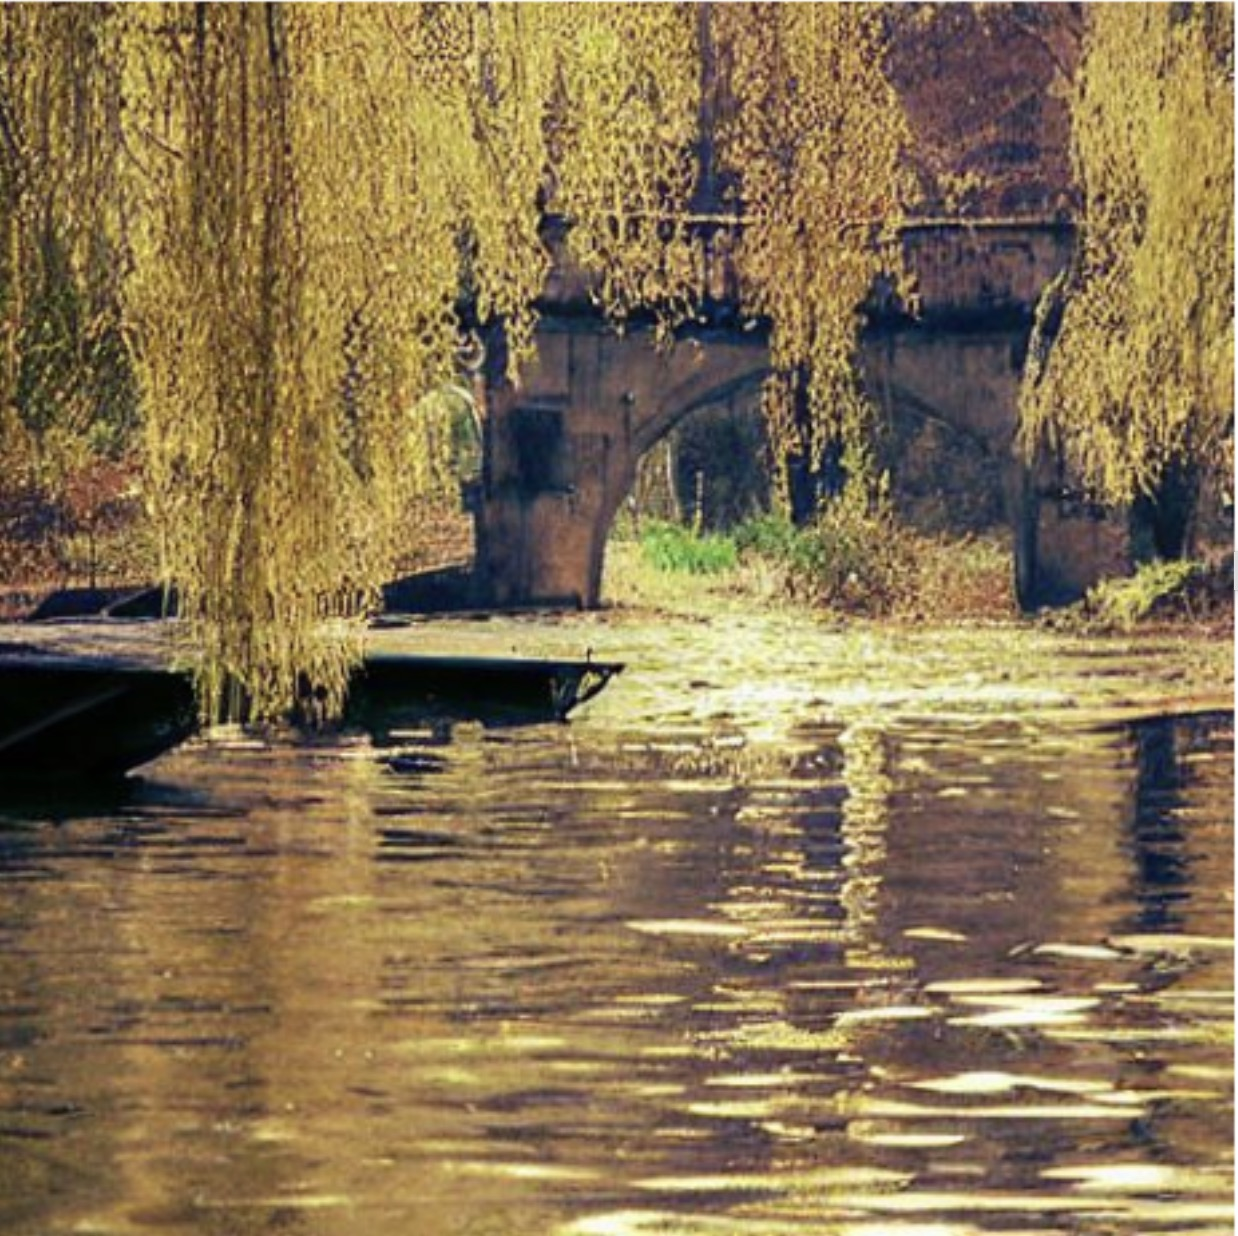
\includegraphics[width=\linewidth]{poster/assets/pic1.png}
         \small\textbf{Image 1: Removing People} 
    \end{minipage}
    \hfill
    \begin{minipage}[t]{0.4\linewidth}
        \centering
        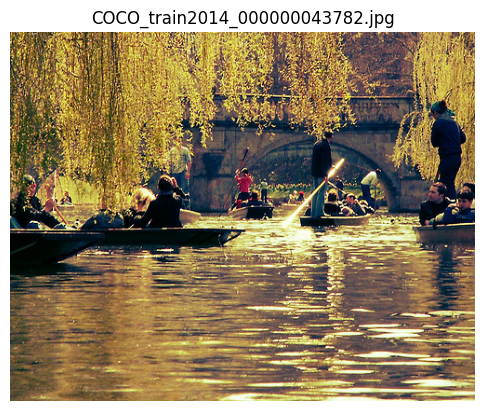
\includegraphics[width=\linewidth]{poster/assets/pic2.png}
        \vspace{0.3em}
        \small\textbf{Image 2: Original} 
    \end{minipage}

Image $1$ similarity (Original CLIP): 0.3248,
Image $1$ similarity (DeCLIP): \textbf{0.4197}\\
Image $2$ similarity (Original CLIP): 0.2788,
Image $2$ similarity (DeCLIP): \textbf{0.1250}\\
\end{block}

    
  
  \begin{block}{Ongoing and Future Work}
    \begin{minipage}[t][20cm][t]{\linewidth}
      % ← 5 cm reserved here for Conclusion
    Now we have automated the process and finished generation of dual imgaes and dual captions of 5,000 training examples together with correspondng fine-tune training of DeClip. Current trend shows that.
    The resulting dual images and texts enrich training with both false and new positive pairs, boosting model robustness.
    \vspace{0.5em}
    \begin{exampleblock}{Ongoing}
    \begin{itemize}
        \item \textbf{Scalability And Efficiency:} Keep on generating dual images and texts for the whole COCO dataset, and optimize the pipeline for large-scale datasets (e.g., 3M images), balancing computational cost and inpainting quality.
        \item \textbf{Benchmark:} Soon after we finished the process of the whole COCO dataset, We will evaluate DeCLIP's zero-shot capability on small-scale datasets such as CIFAR-100 and STL-10, as well as on ImageNet; and compositional reasoning ability using the ARO benchmark.(Till today, we have already seen a bit improvement.)
    \end{itemize}
    \end{exampleblock}

    \end{minipage}
  \end{block}
  

\end{column}


  


\separatorcolumn
\end{columns}
\end{frame}

\end{document}
